\chapter{Design and Implementation}
\section{Proposed Architecture}
\subsection{Concepts of DeAr}
\indent 
One of key features in the DeAr DSP is manipulating Simultaneous Multi-threading (SMT) in each processing core with the purpose of exploiting arithmetic resources.
By dispatching two instruction streams that manipulate its VLIW-fashion datapath, 
the computational workload of a work-item can be amortized by two threads simultaneously.
Figure~\ref{fig:bb:1} illustrates the typical execution flow of an HSA work-item across several basic blocks, 
which refer to piece of code without any branch or jump instruction except at its entry or exit.
The life cycle of the work-item involves executing instructions within a block sequentially, and shuttling among the blocks.
DeAr achieves the speedup by exploiting ILP in each basic block, as shown in Figure~\ref{fig:bb:1}. 
At the entry of a program, two DeAr threads are forked by the hardware in replacement of a work-item.
Next, the forked DeAr threads simultaneously fetch and execute the statically-scheduled instructions to exploit ILP within the basic block.
They join at the end of the basic block, and perform an identical branch or jump instruction targeting the next basic block simultaneously.
The fundamental challenge in SMT is scheduling threads, 
which can be resolved by either hardware (dynamic scheduling) or software (static scheduling).
We applied the latter because the static approach offers more optimization opportunities in scheduling, 
and hardware resources can be dedicated to arithmetics.
\vspace{\textfig}
\begin{figure}[!ht]
    \begin{center}
        \subfigure[Execution flow of an HSA work-item]
        {
            \label{fig:bb:1}
            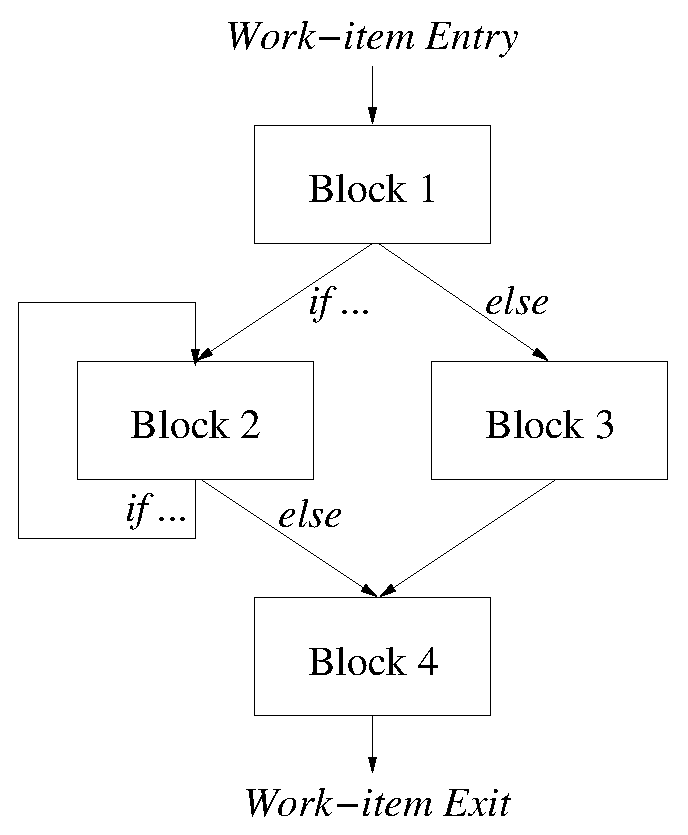
\includegraphics[width=0.3\textwidth]{figs/bb.eps}
        }
        \hfill
        \subfigure[Accelerating the execution of a Basic block]
        {
            \label{fig:bb:2}
            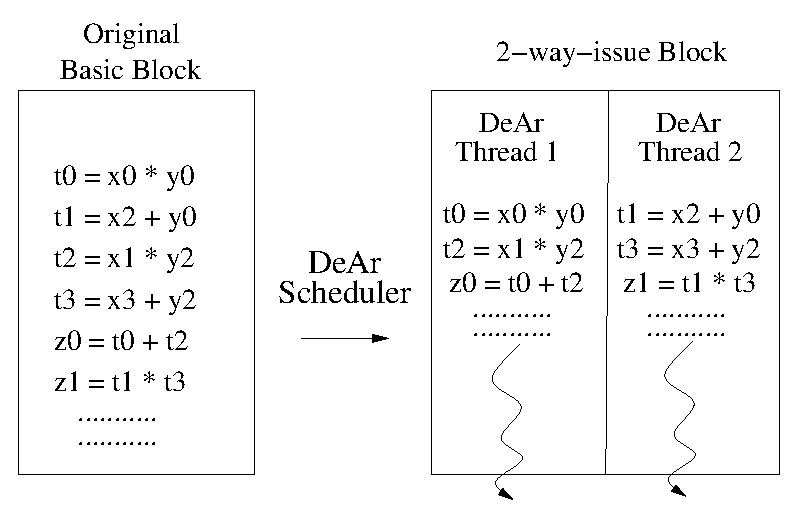
\includegraphics[width=0.55\textwidth]{figs/bb2.eps}
        }
    \end{center}
    \caption{Accelerating HSA with DeAr}
    \label{fig:bb}
\end{figure}
\\\indent 
Another feature is exhaustively compacting the hardware resources while keeping the flexibility and computational power.
This offers the DeAr DSP better efficiency in several perspectives including power consumption, chip area and memory usage.
Moreover, such compact hardware design equips it with excellent scalability, 
which makes DeAr very suitable for the HSA programming model.
A DeAr core can be scaled up to multi-core architecture, 
where the assembly of cores forms the wavefront which supports the HSA SPMD programming model.
\subsection{System Integration}
Figure~\ref{fig:archi} illustrates the example framework of an HSA system integrated with a 4-core DeAr DSP.
The general purpose processor (GPP) hosts OS and HSA runtime, sharing main memory with the DeAr DSP.
In the DSP, each core owns a private L1 D-cache, and shared a L1 I-cache with another.
The L1 I-cache sharing mechanism was proposed in~\cite{kelly2004shared},
which reduces the duplication of program memory in the SPMD model.
The bus interface of the DSP comprises two components, the smart controller (SC) and host port interface (HPI).
SC, proposed by Hsu \textit{et al.}, is a specialized bus interface IP applied to heterogeneous systems.
SC not only performs direct memory access (DMA) for the DSP local memory,
but also re-organize the non-coalescing data transparently to improve the data locality.
On the other hand, HPI, which is a common module found in Texas Instruments DSPs~\cite{hpi},
It facilitates the direct access from the GPP to DSP internal resources with purposes below:
\begin{itemize}
    \item \textbf{MMU}: The host OS accesses the MMU via HPI, and thus HSA SVM can be facilitated.
    \item \textbf{Dispatch queues}: HSA runtime pushes (pops out) AQL-packets to (from) the kernel-dispatch queue (agent-dispatch queue) via HPI, 
        and thus HSA user-mode queuing can be facilitated.
    \item \textbf{SC}: The SC user API sends control signal to SC via HPI, 
        and thus the data transfer and conversion fashion can be specified by the user.
\end{itemize}




\vspace{\textfig}
\begin{figure}[!ht] 
    \centering
    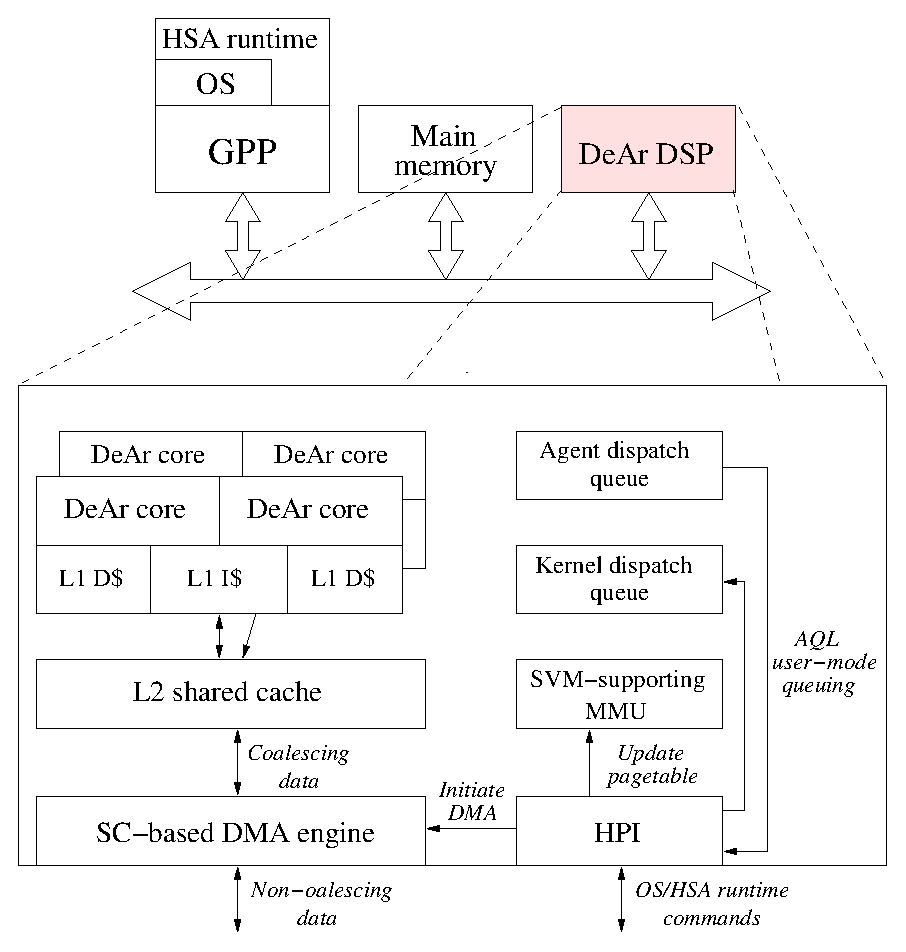
\includegraphics[width=0.8\textwidth]{./figs/archi.eps}
    \caption{Micro-architecture of a DeAr DSP lane}
    \label{fig:archi}
\end{figure}


%To sum up, Each HSA work-item can be summited to a DeAr core and accelerated by two DeAr threads.
%to meet the computational demands of data-intensive applications, such as baseband demodulation and multi-media.


\section{Hardware Design and Implementation}
\subsection{Micro-architecture Design}
% todo program cache, data cache
In this section, we will look into DeAr from a micro-architecture perspective, and explore its design considerations at the same time.
Figure~\ref{fig:micro} illustrates the micro-architecture of DeAr DSP lane.
We adopted the concept of Harvard architecture, 
which separates data memory and instruction memory physically\cite{harvard}.
As a result, the datapath and the control path are wrapped by two independent interfaces, the load/store unit and the instruction unit, respectively.
Such orthogonality between data and instructions offers better freedom of optimizing data precision or code density.
The load/store unit supports burst mode transfer, which enable consecutive fetch of the data in the memory.
This mechanism reduce the number of memory access instructions to be used, 
and improve the utilization of the bus bandwidth.
In addition, DeAr allows the memory transfer to be initiated by two threads orthogonally under the hardware arbitration.
On the other hand, since two DeAr threads always branch simultaneously to the same basic block, 
the compiler can align their simultaneous instructions to adjacent addresses.
As a result, the instruction unit can serve two DeAr threads by doubling the fetch width instead of duplication of the hardware.
\\\indent
Next, we are looking into the datapath.
Two DeAr threads in a lane not only share group of arithmetic units that commonly exist in a RISC datapath, 
but also the same instruction unit which is suitable for synchronous branch.
The demonstrated example includes an adder, a multiplier and a barrel shifter, which are qualified to perform most benchmarks,
Nevertheless, the configuration of arithmetic units can be modified to fit the target applications.
The output of each arithmetic unit is an accumulator register, 
which bypasses the result to any arithmetic units that need it in the next clock cycle.
The bypassing-mechanism of accumulator registers avoid unnecessary accesses to the register file, 
and thus reduce the energy dissipation in the register file.
In addition, the accumulator registers are all clock-gated.
This enables DeAr to preserve the data in accumulator registers until the corresponding arithmetic unit is activated next time, 
offering more data bypassing opportunities.
The bypassing mechanism and resolution of structural hazards are both handled by the software, 
so the hardware complexity of dynamic scheduling or bypassing units can be avoided or reduced.
\\\indent
The register file is physically and symmetrically divided for two DeAr threads.
Each of them owns a pair of queue memory as well as stack memory, 
and these memory units of two DeAr threads thus form the sequential-accessed banked register file (SBRF).
The banked organization of the SBRF cuts off redundant connectivity among read/write ports and register cells.
Compared with the conventional centralized organization, 
the wire area, power consumption and access time of the banked organization are significantly improved, as discussed in Section~\ref{sec:rfcell}.
A queue pair, composed of a load-queue and a store-queue, 
serves as the buffer that connects the lower level of the memory hierarchy with the datapath.
A load-queue and a store-queues can be accessed from their both sides concurrently in the first-in-first-out (FIFO) fashion.
A DeAr thread reads input data from its load-queue and writes the result of computation to its store-queue, 
while the load/store unit accesses the queues in the opposite direction.
By preventing a queue from empty or full with clever scheduling, the latency of load/store via it can thus be hidden.
The stack memory, on the other hand, is responsible for the storage of intermediate data and load/store address.
Other possible uses of the stack memory include branch condition evaluation and returning from interruption.
The nature of a stack memory is last-in-first-out (LIFO), 
which is the key property of the DeAr scheduling algorithm (elaborated in Chapter~\ref{cha:software}).
Applying sequential-access memory units instead of random-access ones effectively reduces the control signal size and decode overhead, 
since any access to the SBRF can be simplified to "PUSH" or "POP".
Such simplification gains high code density and save the wiring from the instruction unit to SBRF, 
and constitute the key advantage of DeAr over conventional VLIW architectures.
For clarity, we summarize the classification of various data registers in the datapath in Table~\ref{tab:register}.
\begin{table}[!ht]
    \caption{Classification of data registers in DeAr}
    \label{tab:register}
    \centering
    \begin{tabular}{|l|l|l|}
        \hline
        \multicolumn{1}{|c|}{\textbf{Register type}} & \multicolumn{1}{c|}{\textbf{Dedicated to}} & \multicolumn{1}{c|}{\textbf{Description}}                 \\ \hline
        Load-queue                                   & \multirow{3}{*}{a DeAr thread}             & buffers input data received from the main memory          \\ \cline{1-1} \cline{3-3} 
        Store-queue                                  &                                            & buffers output data sent to the main memroy               \\ \cline{1-1} \cline{3-3} 
        Stack                                        &                                            & buffers intermediate data of computation                  \\ \hline
        Accumulator                                  & an arithmetic unit                         & buffers the arithmetic result of the previous clock cycle \\ \hline
    \end{tabular}
\end{table}
\\\indent
The design of transport triggered data bus (TTDB) was inspired by TTA~\cite{tta}.
TTDB separates the RF from arithmetic units with a set of multiplexers controlled by the instruction unit, 
and bypasses data from arithmetic units and accumulators.
Possible routes of data over TTDB are summarized as below:
\begin{itemize}
    \item Each arithmetic unit receives the first operand from a load-queue or an accumulator, 
        and receives the second one from a load-queue or a stack.
    \item Each store-queue receives data from the output of an arithmetic unit.
    \item Each stack receives data from the output of an arithmetic unit.
\end{itemize}
\indent
It is important to note that, even though the communication among the RF, arithmetic units and accumulator registers is compacted exhaustively, 
the datapath flexibility is still be kept.
The organization of TTDB is tightly coupled with the instruction set architecture (ISA).
Accordingly, further reduction in instruction size can be achieved with such a compact design.
More insight into the relation between TTDB and ISA will be available in Section~\ref{sec:isa}.

\vspace{\textfig}
\begin{figure}[!ht] 
    \centering
    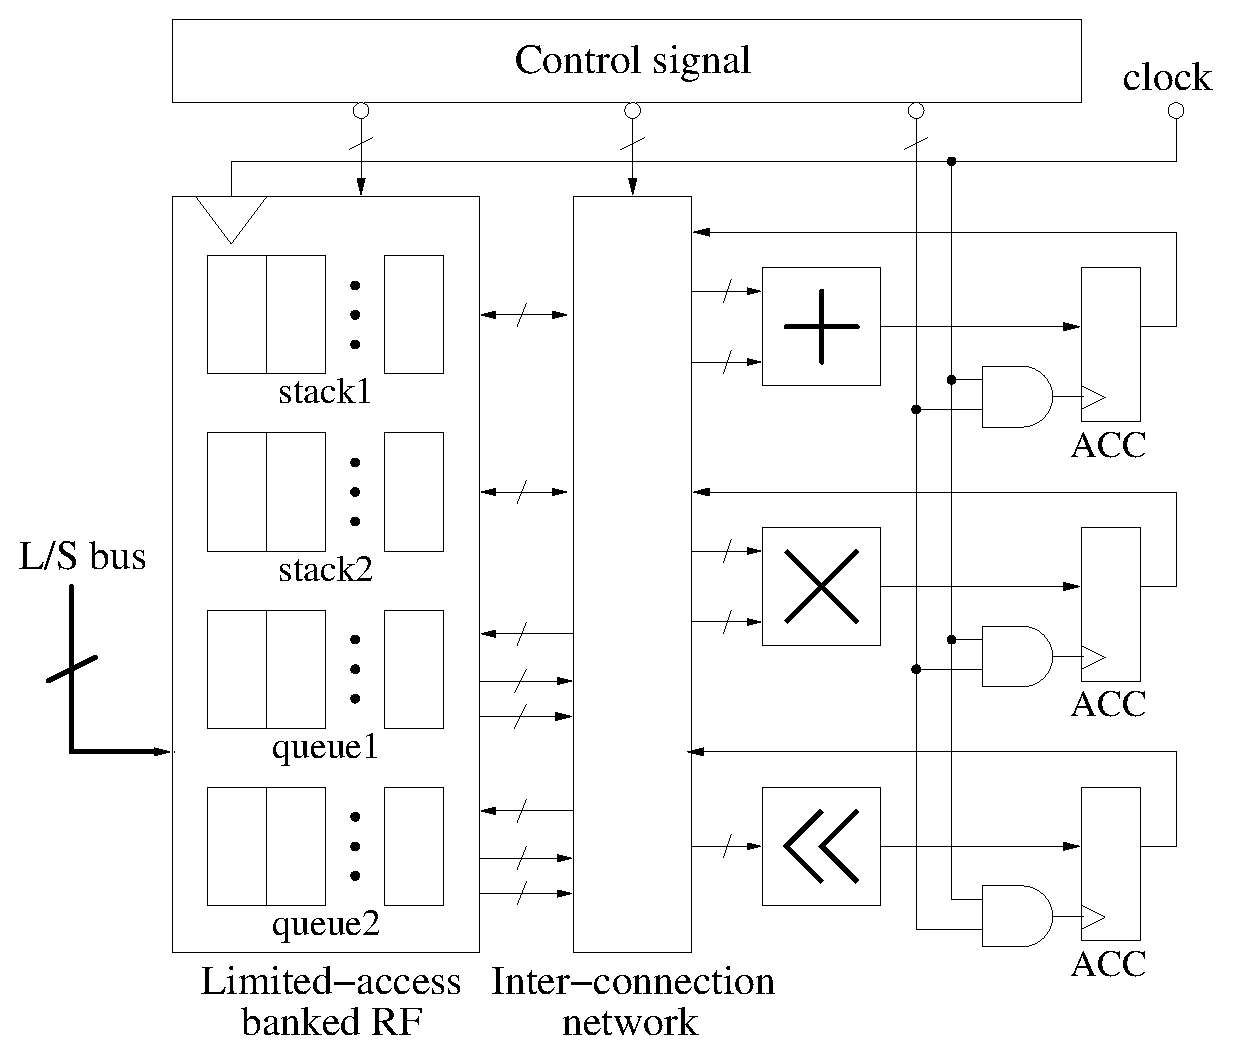
\includegraphics[width=0.85\textwidth]{./figs/micro.eps}
    \caption{Micro-architecture of a DeAr DSP lane}
    \label{fig:micro}
\end{figure}


\subsection{Instruction Set Architecture}
\label{sec:isa}
\indent The DeAr instruction set architecture (ISA) seemingly follows the principle of RISC, which takes instructions with fixed length, 
but the former is optimized for efficient arithmetic.
Each DeAr instruction is composed of two portions, RISC-style portion and stack-access portion.
%The instruction unit issues two instructions simultaneously for two DeAr threads.
Table~\ref{tab:risc} shows the functions of the RISC-style portion, which are similar to some subset conventional RISC ISA.
Here, we use the bold alphabets, \textbf{r}, \textbf{s}, \textbf{t}, \textbf{k}, \textbf{a}, 
to represent the instruction decode bit-fields and illustrate the meaning of each function.
According to their functions, they can be classified to three categories, A type, B type and M type.
A type includes arithmetic instructions such as addition (ADD or SUB), multiplication (MUL) and shift operation (SHL or SHR).
Other instructions like move (MV), which moves data from the other DeAr thread, 
and no operation (NOP), which stalls the DeAr thread for a cycle, 
belong to A type as well since they also manipulate arithmetic units.
B type includes instructions which interact with the instruction unit, such as branch on zero (BE), branch on nonzero (BNE) and unconditional branch (JMP).
M type, on the other, includes memory transfer instructions, load (LD) and store (ST), which manage the load/store unit.
%---------- risc-style portion table
\begin{table}[ht!]
    \centering
    \caption{RISC-style portion of the DeAr instruction set}
    \label{tab:risc}
    \begin{tabular}{|c|l|l|c|}
        \hline
        \multicolumn{1}{|c|}{\textbf{Category}} & \multicolumn{1}{c|}{\textbf{Name}} & \multicolumn{1}{c|}{\textbf{Meaning}} & \multicolumn{1}{c|}{\textbf{Target}} \\ \hline
    \multirow{7}{*}{ \begin{tabular}[c]{@{}l@{}} \\ A type \end{tabular}}      & ADD & \textbf{d} = \textbf{s} + \textbf{t}  & \multirow{7}{*}{\begin{tabular}[c]{@{}l@{}} \\ Datapath \end{tabular}}  \\ \cline{2-3}
                                                                               & SUB & \textbf{d} = \textbf{s} - \textbf{t} & \\ \cline{2-3} 
                                                                               & MUL & \textbf{d} = \textbf{s} * \textbf{t} & \\ \cline{2-3} 
                                                                               & SHL & \textbf{d} = \textbf{s} << \textbf{t} & \\ \cline{2-3}
                                                                               & SHR & \textbf{d} = \textbf{s} >> \textbf{t} & \\ \cline{2-3}
                                                                               & MV  & \textbf{d} = \textbf{s} + 0 or \textbf{d} = \textbf{s} << 0 & \\ \cline{2-3} 
                                                                               & NOP & \begin{tabular}[c]{@{}l@{}}1. disable write back \\ 2. clock-gate the accumulator \end{tabular}& \\ \hline
    \multirow{3}{*}{ \begin{tabular}[c]{@{}l@{}} \\ \\ B type \end{tabular}}          & JMP & pc = pc + \textbf{a}  & \multirow{3}{*}{ \begin{tabular}[c]{@{}l@{}} \\ \\ Instruction unit \end{tabular}} \\ \cline{2-3}
                                                                                      & BZ  & \begin{tabular}[c]{@{}l@{}} \textit{if}(stack1.read() == stack2.read())\\ \ \ \ \ \ \ \ pc = pc + \textbf{a} \end{tabular} & \\ \cline{2-3}
                                                                                      & BNZ & \begin{tabular}[c]{@{}l@{}} \textit{if}(stack1.read() != stack2.read())\\ \ \ \ \ \ \ \ pc = pc + \textbf{a} \end{tabular} & \\ \hline
    \multirow{2}{*}{ \begin{tabular}[c]{@{}l@{}} \\ M type \end{tabular}}           & LD  & \begin{tabular}[c]{@{}l@{}} \textit{repeat}(\textbf{r})\\ \ \ \ \ \ \ \ load\_queue.push (memory[\textbf{a}]) \end{tabular}& \multirow{2}{*}{\begin{tabular}[c]{@{}l@{}} \\  Load/store unit \end{tabular}} \\ \cline{2-3} 
                                                                                    & ST  & \begin{tabular}[c]{@{}l@{}} \textit{repeat}(\textbf{r})\\ \ \ \ \ \ \ \ memory[\textbf{a}] = store\_queue.pop() \end{tabular}& \\ \hline
    \end{tabular}
\end{table}
%-----------------------------------------

\indent 
On the other hand, the stack-access portion, illustrated in Table~\ref{tab:stack}, 
is dedicated to manipulate the stack memory of the DeAr thread.
The possible uses
Four stack operations, PUSH, POP, MODIFY and NOP, are defined, 
Each DeAr thread uses these stack operations to buffer its data in the LIFO manner.
A PUSH operation stores the result from one of arithmetic units and adds the head address by 1, 
while a POP operation eliminate the head data by subtracting the head address by 1.
Since a POP operation followed by a PUSH operation modifies the data at the head data and maintains the head address, 
a MODIFY operation is defined to simplify the usage of two operations.
In some scenarios, the DeAr thread does nothing to the stack but keeps its condition.
As a result, a NOP operation is also defined for the stack-access portion.
Note that the NOP of stack-access portion should be distinguished from the one of RISC-style portion.
These two portions constitute DeAr ISA.
The DeAr thread can thus access an arithmetic units with the RISC-style portion and handle the intermediate result with stack-access portion.
On the other hand, since the memory transfer instructions (i.e., LD and ST) never generate intermediate, 
they do not need the stack-access portion.
We can thus preserve more bits in the memory transfer instruction to address larger memory space.

%---------- stack portion table
\begin{table}[ht!]
    \centering
    \caption{Stack access portion of the DeAr instruction set}
    \label{tab:stack}
    \begin{tabular}{|l|l|l|}
        \hline
        \multicolumn{1}{|c|}{\textbf{Name}} & \multicolumn{1}{c|}{\textbf{Meaning}} & \multicolumn{1}{c|}{\textbf{Note}} \\ \hline
    PUSH & \begin{tabular}[c]{@{}l@{}}1. Add the head address by 1\\ 2. Write the new data to the head address\end{tabular} & \multirow{2}{*}{ \parbox{5cm}{A "pop" followed by a "push" is equivalent to a "modify"} } \\ \cline{1-2}
    POP                               & \begin{tabular}[c]{@{}l@{}}1. Subtract the head address by 1\\ 2. Invalidate the previous head data\end{tabular} & \\ \hline
        MODIFY                            & Modify the head data to to the new data & The head address remains \\ \hline
        NOP                               & No operation & The head address and data remain \\ \hline
    \end{tabular}
\end{table}
%-----------------------------------------

Each DeAr instruction is 12-bit in length.
To offer better insight into the instruction decode mechanism, 
Table~\ref{tab:decode} elaborates three instruction types, 
each of which is enumerated from MSB to LSB.
Marks of the first column represent various bit-fields, 
and they correspond to the bold alphabets shown in Table~\ref{tab:risc}.
%Note that Table~\ref{tab:decode} also reveals the detailed organization of the TTDB by elaborating the communication in the datapath.
A-type instruction include all arithmetic instructions.
The head 4-bit signal \textbf{f}, which is similar to the function code in RISC, specifies the operation to be performed.
It is followed by a single-bit signal \textbf{d}, which determines whether the result of this operation is written back to the memory via the store-queue.
After that, a pair of 2-bit signals, \textbf{s} and \textbf{t}, select the sources of two arithmetic operands respectively. 
Nevertheless, the data sources selected by \textbf{s} and \textbf{t} are not identical.
The former selects the first operand from the load-queue or one of accumulator registers, 
while the latter selects the second one from the load-queue, stack, or constants (1 or 0).
Some instructions like SHR and SHL use immediate constants as the second operand (i.e., shifting amount).
In such a scenario, \textbf{t} and the reserved bit serve as immediate data.
Finally, the last 2-bit \textbf{k} is the stack access portion, which encodes four operations that manipulate the stack memory.
Note that the functions of \textbf{f} and \textbf{k} remain in M type and B type.
\\\indent On the other hand, M-type instructions perform memory transfers.
The function field \textbf{f} is followed by 2-bit signal \textbf{w}, 
which specifies the word size of the transfer.
The size can be byte (8-bit), halfword (16-bit) or word (32-bit).
Another bit value \textbf{b} indicates whether the memory transfer is performed in the burst mode, 
and the following 2, \textbf{r}, determines the length of the burst (i.e., the number of transfers to be performed consecutively).
The burst length can be 2, 4, 8 or 16.
If \textbf{b} is de-asserted, \textbf{r} will be ignored.
\\\indent The last category, B-type instructions, which control the program flow, 
is a special case compared with the previous two.
Since two DeAr threads always perform identical branch instructions simultaneously, 
two branch instructions can be merged into one with more bits for branch target addressing.
As a result, B-type instructions can manipulate 24-bit, which is twice of the original one in length.
The function field \textbf{f} is followed by 16-bit branch address offset \textbf{a}.
%Likewise, the last 2-bit \textbf{k} denotes the stack access portion, which follows unused 2 bits.

%---------- bit field table---------------
\begin{table}[!ht]
    \centering
    \caption{Instrucion decode table of the DeAr instrucion set}
    \label{tab:decode}
    \begin{tabular}{|l|l|l|}
        \hline
        \multicolumn{1}{|c|}{\textbf{Mark}} & \multicolumn{1}{c|}{\textbf{Bit field}} & \multicolumn{1}{c|}{\textbf{Description}} \\ \hline
        \multicolumn{3}{|c|}{\textbf{A-type instructions}} \\ \hline
    f & {[}11:8{]} & \begin{tabular}[c]{@{}l@{}}Select the function from ADD, SUB, SHL, SHR, MUL, MV or NOP\end{tabular} \\ \hline
    d & {[}7{]} & \begin{tabular}[c]{@{}l@{}}Enable WB to the store-queue\end{tabular} \\ \hline
    s & {[}6:5{]} & \begin{tabular}[c]{@{}l@{}}Select the first operand from load-queue or accumulators \end{tabular} \\ \hline
    t & {[}4:3{]} & \begin{tabular}[c]{@{}l@{}}1. Select the second operand from load-queue, stack, constant 0 or 1 \\ 2. Immediate data for SHR or SHL\end{tabular} \\ \hline
    - & {[}2{]} & \begin{tabular}[c]{@{}l@{}}1. Reserve \\ 2. Immediate data for SHR or SHL\end{tabular} \\ \hline
    k & {[}1:0{]} & \begin{tabular}[c]{@{}l@{}}Stack access portion\end{tabular} \\ \hline
        \multicolumn{3}{|c|}{\textbf{M-type instructions}} \\ \hline
    f & {[}11:8{]} & \begin{tabular}[c]{@{}l@{}}Select the function from LD or ST\end{tabular} \\ \hline
    %e & {[}7{]} & \begin{tabular}[c]{@{}l@{}}Specify the endianness of the data in the memory \end{tabular} \\ \hline
    w & {[}7:6{]} & \begin{tabular}[c]{@{}l@{}}Select the word size from byte, halfword or word \end{tabular} \\ \hline
    b & {[}5{]} & \begin{tabular}[c]{@{}l@{}}Enable burst mode memory transfer \end{tabular} \\ \hline
    r & {[}4:3{]} & \begin{tabular}[c]{@{}l@{}}Select the burst length from 2, 4, 8 or 16 \end{tabular} \\ \hline
    - & {[}2{]} & \begin{tabular}[c]{@{}l@{}}Reserve \end{tabular} \\ \hline
    k & {[}1:0{]} & \begin{tabular}[c]{@{}l@{}}Stack access portion\end{tabular} \\ \hline
        \multicolumn{3}{|c|}{\textbf{B-type instructions}} \\ \hline
    f & {[}23:20{]} & \begin{tabular}[c]{@{}l@{}}Select the function from BE or BNE\end{tabular} \\ \hline
    a & {[}19:4{]} & \begin{tabular}[c]{@{}l@{}}Specify the branch address offset \end{tabular} \\ \hline
    - & {[}3:2{]} & \begin{tabular}[c]{@{}l@{}}Reserve \end{tabular} \\ \hline
    k & {[}1:0{]} & \begin{tabular}[c]{@{}l@{}}Stack access portion\end{tabular} \\ \hline
    \end{tabular}
\end{table}
%------------------------------------------


\section{Software Design and Implementation}
\label{sec:software}
\subsection{Software framework for DeAr}
\label{sec:software:framework}
To fully exploit the power of DeAr, we also present a completed code generation flow including compilation, scheduling and optimization.
Algorithm~\ref{alg:framework} provides an overview of the software framework for DeAr. 
The user only need to provide DSP kernel code written in OpenCL and a flag which determines the optimization level as the input.
With CLOC \cite{cloc} tool provided by \textit{HSA Foundation}, the kernel code is converted to standardized HSAIL, $H$, as shown in Line~\ref{line:tohsail}.
Next, in Line~\ref{line:trans}-\ref{line:trane}, 
we run the HSAIL transformation (elaborated in \ref{sec:trans}) on HSAIL code and obtain a hierarchical data flow graph (HDFG), 
$\bar{G}$ (elaborated in \ref{sec:hdfg}), which holds crucial scheduling heuristics.
After that, in Line~\ref{line:optstart} to \ref{line:optend}, we perform the key part of DeAr software, 
operation scheduling and optimization (elaborated in \ref{sec:sando}).
The optimization flag $\lambda$ in Line~\ref{line:forlambda} determines the number of iterations to be used.
For each iteration, the scheduler exhausts heuristics in $\bar{G}$ which optimize the cycle and WB counts, 
and it schedules operations with a limited randomness.
Finally, the scheduler select the scheduling result with the least cycle count, 
$C_{golden}$ among iterations and generates the final code $X_{golden}$ for DeAr as the output.
%-----------------framework algo -------------
\begin{algorithm}[h]
    \caption{\textproc{Software Framework for DeAr}}
    \begin{algorithmic}[1]
        \Require 
        High-level DSP kernel code in OpenCL, Optimization flag $\lambda$
        \Ensure 
        Binary code of DeAr

        %\State Convert the kernel code to HSAIL code
        \State $hsail \Leftarrow$ \Call{CL Offline Compiler }{ $kernel$ }
        \label{line:tohsail}
        %\State Perform SSA transformation on HSAIL;
        %\label{tossa}
        %\State Convert SSA code to DFG, $G = ( V_{op} , E_{op} )$, where $V_{op}$ is the set of operations and $E_{op}$ is the set of their dependencies;
        %\label{todfg}
        %\State Perform hierarchization on $G$, and get $\bar{G} = ( V_{bt} , E_{bt} )$, where $V_{bt}$ is a set of binary trees and $E_{bt}$ is the set of their dependencies;
        \State $G \Leftarrow$ \Call{Convert HSAIL to DFG by SSA }{ $hsail$ }
        \label{line:trans}
        \State $\bar{G} \Leftarrow$ \Call{Hierarchize DFG to HDFG }{ $G$ }
        %\State Perform the HSAIL transformation on HSIL code, and obtain a HDFG, $\bar{G}$
        \label{line:trane}
        \State $C_{golden} \Leftarrow  \infty$
        \label{line:optstart}
        \For {$i=1$ to $f(\lambda)$}
        \label{line:forlambda}
        %\State Schedule operations in $\bar{G}$ and get binary code $X_i$ and its total cycle count $C_i$
        \State $X_{inter}, bt_{remain} \Leftarrow$ \Call{Inter-tree Scheduling }{ $\bar{G}$ }
        \State $X_i, C_i \Leftarrow$ \Call{Intra-tree Scheduling }{ $X_{inter}, bt_{remain}$ }
        \If {$C_i < C_{golden}$}
        \State $C_{golden} \Leftarrow C_i$
        \State $X_{golden} \Leftarrow X_i$
        \EndIf
        \EndFor
        \State Return $X_{golden}$
        \label{line:optend}
    \end{algorithmic}
    \label{alg:framework}
\end{algorithm}
%-----------------------------------------

\subsection{Data Flow Graph and Hierarchical Data Flow Graph}
\label{sec:hdfg}
A data flow grahp (DFG), which presents dependencies among operations, is crutial information for program analysis.
By partitioning a program into basic blocks, the control flow can be simplified, and thus each DFG of a basic block is a directed acyclic graph (DAG).
Figure~\ref{fig:dfg:dfg} illustrates an example of a DFG, where each node and each edge denote an operation and a dependency respectively.
We can further express any DFG as a data structure $G$, which holds a set of nodes (operations), $V_{op}$, and a set of edges (dependencies), $E_{op}$
In conventional DSP software design, optimal scheduling of operations is often approached by analyzing DFGs.
For example, \cite{dsplite} solves ILP problems \cite{ilp} in DFGs in scheduling, 
and list scheduling \cite{list} calculates scheduling range of operations in DFGs as the scheduling criteria. 
\\\indent
However, we found that conventional DFG analysis is infeasible for scheduling in DeAr due to uniqueness of its datapath.
As a result, in this work, we propose an enhanced version of DFG, hierarchical data flow graph (HDFG), to fit DeAr datapath.
Figure~\ref{fig:dfg:hdfg} demonstrates an HDFG, $\bar{G} = {V_{bt}, E_{bt}}$, converted from Figure~\ref{fig:dfg:dfg}.
We enumerate several important features of HDFG as below: 
\begin{itemize}
    \item Cascaded operations, which implies no fork and join of edges within the cascade, are grouped into a super node ($sn$). 
        If an operation is isolated, it forms a $sn$ directly.
    \item Neighboring $sn$ are further grouped into binary trees, $bt$s, which form a set of vertices, $V_{bt}$, in HDFG.
        If a $sn$ is isolated, it forms a binary tree directly.
    \item Dependencies among operations that cross binary trees are inherited by binary trees they belong to.
        These inherited dependencies form a set of edges, $E_{bt}$, among $V_{bt}$.
    \item A $bt$ without any in-edge existing in $V_{bt}$ (i.e., $\sum_{v \in V_{bt}}\textrm{deg}^-(bt) = 0$) is free to be scheduled. 
        After scheduled, the $bt$ and its edge will be erased from $\bar{G}$.
    \item Every $sn$ must have either zero (leaf nodes) or two (non-leaf nodes) children.
        Edges in a HDFG at $bt$, $sn$ and operation level guarantee the correctness of execution order.
\end{itemize}
\indent The hierarchy of HDFGs can provide crutial optimization heuristics to the DeAr scheduler.
DeAr avoids RF access within each super node, and regularize RF access into first-in last-out fashion (stack) with the help from the recursive property of a binary tree.
Moreover, the binary property also provides more opportunities to balance workload of two threads, and thus higher OPC can be achieved.
\vspace{\textfig}
\begin{figure}[!ht]
    \begin{center}
        \subfigure[DFG example]
        {
            \label{fig:dfg:dfg}
            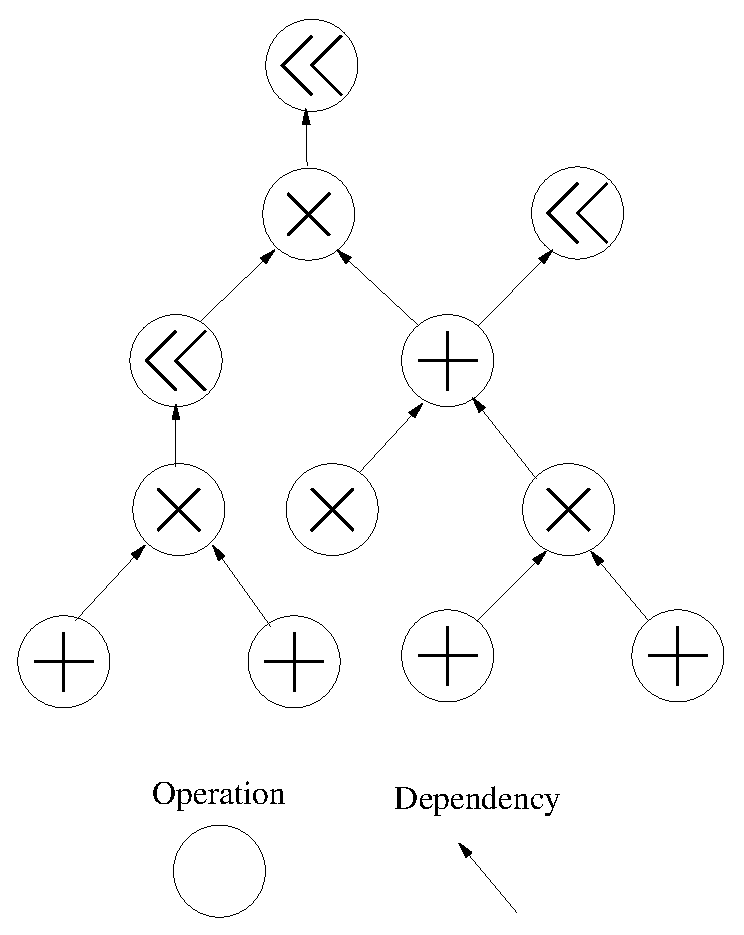
\includegraphics[width=0.45\textwidth]{figs/dfg.eps}
        }
        \subfigure[Corresponding HDFG]
        {
            \label{fig:dfg:hdfg}
            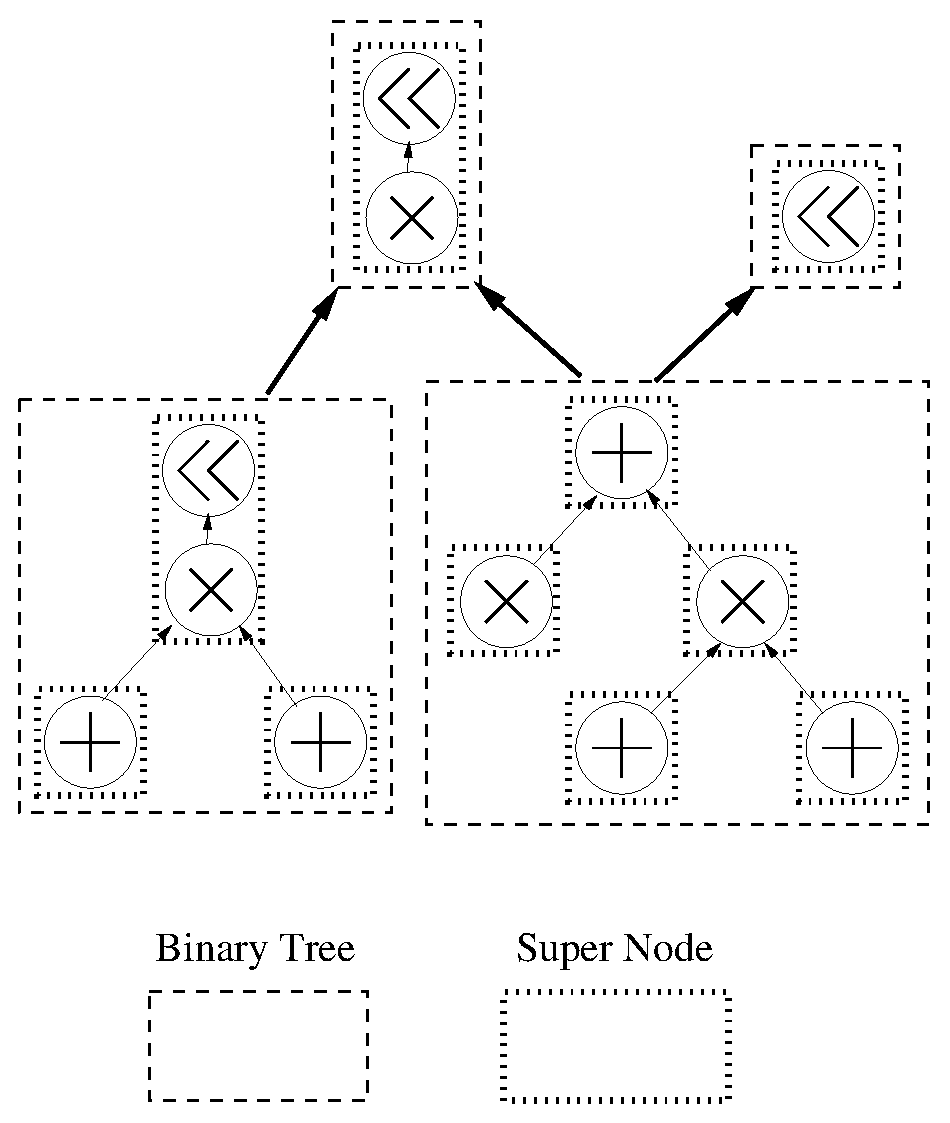
\includegraphics[width=0.45\textwidth]{figs/hdfg.eps}
        }
    \end{center}
    \caption{Conversion from DFG to HDFG}
    \label{fig:dfg}
\end{figure}


\subsection{HSAIL Transformation}
\label{sec:trans}
The whole process of the HSAIL transformation contains two phases elaborated as below:
\begin{itemize}
    \item \textbf{Phase 1: Convert HSAIL to DFG by SSA} \\\indent
        Algorithm~\ref{alg:2dfg} illustrates how this phase works.
        Single static assignment (SSA) \cite{ssa} is another form of IR which simplifies work of compiler significantly, 
        and thus deriving the SSA form of the code becomes the first step.
        SSA form specifies that each variable must be assigned exactly once, which is the key distinction from HSAIL.
        \\\indent
        The conversion from normal HSAIL to SSA form is initialized by performing reaching definition analysis \cite{rda} as shown in Line~\ref{line:rda}.
        Next, for each assignment in the code, we give a new name to the LHS variable, and update corresponding new names of RHS variables indicated by reaching definition analysis.
        These iterations which derive the SSA form correspond to Line~\ref{line:forhsails}-\ref{line:forhsaile}.
        Now, each assignment to some variable $X$ denotes an operation, which dominates operations with $X$ appearing in their RHS variables.
        As a result, we can construct the DFG without burden by iterating the new code, as shown in Line~\ref{line:forssas}-\ref{line:forssae}.
        Operations and their dependencies are stored in a set of vertices $V_{op}$ and a set of edges $E_{op}$ respectively, 
        and thus the DFG, $G = ( V_{op} , E_{op} )$, is constructed.
        %----------hsail to dfg algo--------------
        \begin{algorithm}[ht!]    \caption{\textproc{Convert HSAIL to DFG by SSA}}
            \begin{algorithmic}[1]
                \Require    HSAIL code
                \Ensure     $G = ( V_{op} , E_{op} )$   \Comment{ DFG }
                \State      Peform reaching definition analysis     \label{line:rda}
                \For        {each assignment (operation) in the HSAIL code}     \label{line:forhsails}
                \State      Give a new name to the LHS variable
                \State      Update RHS variables with corresponding new names in other assignments
                \EndFor                                                     \label{line:forhsaile}
                \State      Initialize $G \textrm{, where } V_{op} = \emptyset \textrm{ and } E_{op} = \emptyset $
                \For        {each assignment (operation) in the new HSAIL code} \label{line:forssas}    \Comment{SSA form}
                \State      Insert the LHS variable $x$ to $V_{op}$
                \For        {each variable $y$ in the RHS}
                \State      Insert a new edge ($x$, $y$)
                \EndFor
                \EndFor                                                         \label{line:forssae}
            \end{algorithmic}
            \label{alg:2dfg}
        \end{algorithm}
        %----------------------------------------

    \item \textbf{Phase 2: Hierarchize DFG to HDFG} \\\indent
        As discussed in~\ref{sec:hdfg}, an HDFG is an enhanced version of a DFG which provides necessary heuristics for DeAr scheduler.
        Hierarchizing a DFG to an HDFG can be achieved by traversing the DFG, details of which are shown in Algorithm~\ref{alg:tohdfg}.
        In Line~\ref{line:forroots}-\ref{line:forroote}, the algorithm firstly iterates all root operations (i.e., $\textrm{deg}^+(op)=0$ ) in $G$,
        and call the first subroutine, \textproc{Build Binary Tree }, on each root operations.
        Line~\ref{line:bbts}-\ref{line:bbte} show the details of \textproc{Build Binary Tree }.
        A binary tree $bt$ is initialized by building a super node $sn$ on the input operation $op$ with the second subroutine, \textproc{Build Super Node }, 
        which groups cascaded operations ending with $op$, as shown in Line~\ref{line:bsns}-\ref{line:bsne}.
        After that, the third subroutine \textproc{Grow Binary Tree }, described in Line~\ref{line:gbts}-\ref{line:gbte}, will expand $bt$ by including neighboring operations if each of operations has exactly one out-edge (i.e., $\textrm{deg}^+(op)=1$), as shown in Line~\ref{line:growifs}-\ref{line:growife}. 
        \\\indent
        On the contrary, if the aforementioned condition is not met with any of $op_{left}, op_{right}$, 
        it will call \textproc{Build Binary Tree } on both to build new binary trees, $bt_{left}, bt_{right}$,
        and record the new dependencies, $bt_{left} \rightarrow bt, bt_{right} \rightarrow bt$.
        This step is demonstrated in Line~\ref{line:growelses}-\ref{line:growelsee}. 
        \\\indent
        The recursion proceeds by cross-calling between \textproc{Build Binary Tree } and \textproc{Grow Binary Tree } until the whole DFG is traversed.
        Binary trees and their dependencies are stored in a set vertices $V_{bt}$ and a set of edges $E_{bt}$ respectively.
        Finally, the HDFG, $\bar{G} = ( V_{bt} , E_{bt} )$, is constructed and returned.
\end{itemize}

%----------DFG to HDFG algo--------------
\begin{algorithm}[ht!]    \caption{\textproc{Hierarchize DFG to HDFG}}
    \begin{algorithmic}[1]
        \Require    $G = ( V_{op} , E_{op} )$ \Comment{ DFG }
        \Ensure     $\bar{G} = ( V_{bt} , E_{bt} )$ \Comment{ HDFG }
        \State      Initialize $\bar{G} \textrm{, where } V_{bt} = \emptyset \textrm{ and } E_{bt} = \emptyset $
        \For        {each of $  op \ni \sum_{op \in V_{op}}\textrm{deg}^+(op) = 0 $}  \label{line:forroots}   \Comment{For each root vertex}
        \State      $v_{bt} \Leftarrow $\Call{Build Binary Tree }{$op$}
        \State      Insert $v_{bt}$ to $V_{bt}$
        \EndFor                                                                    \label{line:forroote}
        \Statex %---------------------------
        \Function   {Build Binary Tree }{$op$}         \label{line:bbts}
        \State      Initialize a birary tree $bt$
        \State      $sn \Leftarrow$ \Call{Build Super Node }{$op$}
        \State      Set $sn$ as the root of $bt$
        \State      \Call{Grow Binary Tree }{$sn$}
        \State      \Return {$bt$}
        \EndFunction                                \label{line:bbte}
        \Statex %--------------------------
        \Function   {Grow Binary Tree }{$sn$}          \label{line:gbts}
        \If         { $\textrm{deg}^-(sn.tail) = 2$ }     \Comment{A branch in the DFG}
        \State      $op_{left}, op_{right} \Leftarrow op \ni (op \rightarrow sn.tail) \in E_{op}$ 
        \If         {$\textrm{deg}^+(op_{left}) = \textrm{deg}^+(op_{right}) =1$}  \label{line:deg}  \label{line:growifs}
        \State      $sn.left\_child \Leftarrow$ \Call{Build Super Node }{$op_{left}$}
        \State      \Call{Grow Binary Tree }{$sn_{left}$}
        \State      $sn.left\_child \Leftarrow$ \Call{Build Super Node }{$op_{right}$}
        \State      \Call{Grow Binary Tree }{$sn_{right}$}     \label{line:growife}
        \Else       \label{line:growelses}
        \State      $bt_{new} \Leftarrow$ \Call{Build Binary Tree }{$op_{left}$}
        \State      Insert the new tree $bt_{new}$ to $V_{bt}$
        \State      Insert the new edge $(bt_{new} \rightarrow v_{bt})$ to $bt$
        \State      $bt_{new} \Leftarrow$ \Call{Build Binary Tree }{$op_{right}$}
        \State      Insert the new tree $bt_{new}$ to $V_{bt}$
        \State      Insert the new edge $(bt_{new} \rightarrow v_{bt})$ to $bt$ \label{line:growelsee}
        \EndIf                          \label{line:gbte}
        \EndIf
        \EndFunction
        \Statex %-----------------------
        \Function   {Build Super Node }{$op$}  \label{line:bsns}
        \State  Initialize a super node $sn$ 
        \State  $sn.head \Leftarrow op$
        \While{$\textrm{deg}^-(op) = 1$}
        \State   $op \Leftarrow op_{next} \ni (op_{next} \rightarrow op) \in E_{op}$ 
        \EndWhile
        \State  $sn.tail \Leftarrow op$
        \State      \Return {$sn$}
        \EndFunction                        \label{line:bsne}
    \end{algorithmic}
    \label{alg:tohdfg}
\end{algorithm}
%--------------------------------------


\subsection{Scheduling}

A scheduler is responsible for ensuring the order of operations, 
arranging data movement and allocating hardware resources.
Once the scheduling result is determined, the corresponding machine code is also generated.
The principle of the DeAr scheduler is, 
two threads process binary trees in a HDFG concurrently and collaboratively until all operations are scheduled.
Before exploring how threads co-work, we need to look into how a binary tree, $bt$, is handled by the scheduler.
Algorithm~\ref{alg:sbt}, \textproc{Schedule Binary Tree}, 
demonstrates how operaions of a $bt$ are scheduled into a specific sequence.
%-------Schedule Binary Tree----------
\begin{algorithm}[!ht]
    \caption{\textproc{Schedule Binary Tree }}
    \begin{algorithmic}[1]
        \Require    $sn$
        \Ensure     $list_{op}$
        \If{$sn$ is NOT a leaf node}        \label{line:sbts}
        \State $size_{left} \Leftarrow$ \Call{Stack Size }{$sn.left\_child$}
        \State $size_{right} \Leftarrow$ \Call{Stack Size }{$sn.right\_child$}
        \If{$size_{left} > size_{right}$}
        \State \Call{Schedule Binary Tree }{$sn.left\_child$}
        \Else
        \State \Call{Schedule Binary Tree }{$sn.right\_child$}
        \EndIf
        \EndIf
        \State \Call{Schedule Super Node }{$sn$}   
        \State Erase $sn$ from the binary tree
        \If{$sn$ IS a root node}        
        \State \Return{$list_{op}$}
        \EndIf

        \label{line:sbte}
        \Statex
        \Function   {Stack Size }{$sn$}  \label{line:gsss}
        \If{$sn$ is a leaf node}
        \State $size \Leftarrow 0$
        \Else
        \State $size \Leftarrow \text{\textproc{Max}(\ \textproc{Stack Size }($sn.left\_child$), \textproc{Stack Size }($sn.right\_child$)\ )} + 1$
        \EndIf
        \State \Return{$size$}
        \EndFunction                    \label{line:gsse}
        \Statex
        \Function   {Schedule Super Node }{$sn$}  \label{line:ssns}
        \State   $op \Leftarrow$ $sn.tail$
        \Do   
        \State Insert $op$ to $list_{op}$
        \State $op \Leftarrow op_{next}$
        \DoWhile{$op \neq sn.head$}
        \EndFunction                            \label{line:ssne}

    \end{algorithmic}
    \label{alg:sbt}
\end{algorithm}
%----------------------------------------------
It traverse a $bt$ recursively in a post-order fashion, which implies the root is touched first but scheduled last.
The input is the root $sn$ of a $bt$, and then a list of operations, which indicates execution flow, is returned.
Line~\ref{line:sbts}-\ref{line:sbte} is the main part of the algorithm.
For a input $sn$, the existence of its children is checked at the beginning.
If children exist, the same algorithm, \textproc{Schedule Binary Tree }, is applied to them and the recursion starts.
The first subroutine, \textproc{Stack Size } shown in Line~\ref{line:gsss}-\ref{line:gsse}, determines the precedence of children.
After the recursion, the second subroutine, 
\textproc{Schedule Super Node} shown in Line~\ref{line:ssns}-\ref{line:ssne}, is applied to this $sn$, 
By this subroutine, cascaded operations in the $sn$ are scheduled consecutively.
\\\indent
The key insight of Algorithm~\ref{alg:sbt} is, it optimizes RF access significantly with heuristics from HDFGs.
Firstly, operations in a $sn$ are scheduled consecutively.
With this policy, the forwarding mechanism in DeAr can be taken advantage, and unnecessary WB is can be avoided.
Secondly, the scheduler always schedules the child which demands larger stack size earlier, 
By this mean, the stack size used by a parent $sn$ is the smaller one of two children plus one, 
so that we can ensure the cost on stack size is minimized and prevent RF from spilling.
\\\indent
We further introduce \textproc{Inter-tree scheduling} and \textproc{Intra-tree scheduling}, 
both of which require Algorithm~\ref{alg:sbt}.
A typical HDFG contains multiple $bt$.
As a result, the DeAr scheduler perform \textproc{Inter-tree scheduling} if multiple $bt$ exist.
Algorithm~\ref{alg:inter} illustrate the detail of \textproc{Inter-tree scheduling}, 
where a HDFG, $\bar{G}$ is input, and binary code segment, 
$X_{inter}$, accompanied with a remaining subtree, $bt_{remain}$, will be returned.
%-----------Inter-tree-------------
\begin{algorithm}[ht!]
    \caption{\textproc{Inter-tree Scheduling}}
    \begin{algorithmic}[1]
        \Require    HDFG $\bar{G} = (V_{bt}, E_{bt})$
        \Ensure     Remaining subtree $bt_{remain}$, binary code segment $X_{inter}$
        \State $X_{inter} \Leftarrow NULL$       \Comment{Initialize $X_{inter}$}
        \While{$V_{bt} \neq \emptyset$} \label{line:interws}
        \If{$work\_queue_{thread1} = \emptyset$}
        \State Select a binary tree $bt \ni \sum_{bt \in V_{bt}}\textrm{deg}^-(bt) = 0$ randomly
        \State $list_{op} \Leftarrow$ \Call{Schedule Binary Tree }{$bt.root$}
        \State Push $list_{op}$ into $work\_queue_{thread1}$
        \State Erase $bt$ and its edges from $\bar{G}$
        \EndIf
        \If{$work\_queue_{thread2} = \emptyset$}
        \State Select a binary tree $bt \ni \sum_{bt \in V_{bt}}\textrm{deg}^-(bt) = 0$ randomly
        \State $list_{op} \Leftarrow$ \Call{Schedule Binary Tree }{$bt.root$}
        \State Push $list_{op}$ into $work\_queue_{thread2}$
        \State Erase $bt$ and its edges from $\bar{G}$
        \EndIf
        \State $X_{inter} \Leftarrow X_{inter} \oplus$ \Call{ALU Alloc}{$work\_queue_{thread1}$, $work\_queue_{thread2}$} \label{line:intercon}
        \EndWhile \label{line:interwe}
        \If{$work\_queue_{thread1} \neq \emptyset$} \label{line:interis}
        \State $bt_{remain} \Leftarrow$ \Call{Restore Subtree from Queue }{$work\_queue_{thread1}$}
        \State Clear $work\_queue_{thread1}$
        \ElsIf{$work\_queue_{thread2} \neq \emptyset$}
        \State $bt_{remain} \Leftarrow$ \Call{Restore Subtree from Queue }{$work\_queue_{thread2}$}
        \State Clear $work\_queue_{thread2}$
        \Else
        \State $bt_{remain} \Leftarrow NULL$
        \EndIf \label{line:interie}
        \State \Return{$X_{inter}$, $bt_{remain}$}
    \end{algorithmic}
    \label{alg:inter}
\end{algorithm}
%------------------------------------------
Line~\ref{line:interws}-\ref{line:interwe} enclosed by a while loop, is the main part of \textproc{Inter-tree scheduling}.
The scheduler performs several identical steps for thread~1 and thread~2 respectively.
It firstly search the whole $\bar{G}$ and select a free $bt$ randomly.
Such a selection preserves randomness for DeAr scheduler, 
and a better scheduling result is possible to be achieved with more trials, as discussed in Algorithm~\ref{alg:framework}.
Next, the scheduler checks whether the work-queue of a thread is empty.
If it is empty, the scheduler processes the selected $bt$ with Algorithm~\ref{alg:sbt}, 
and enqueue the returned $op_{list}$ to the work-queue of a thread.
Here, a work-queue is data structure that holds the operation sequence that belongs to a thread.
An operation is removed from a thread's work-queue once it is indeed dispatched to binary code.
After above steps, two work-queue are filled, and the key step of this algorithm, \textproc{ALU Alloc}, is performed.
\textproc{ALU Alloc} dispatches operations in two work-queues which execute concurrently and returns a code segment.
To resolve any resource conflict, it applies Dynamic Programming (DP)~\cite{dp} to allocates ALUs for DeAr thread.
After \textproc{ALU Alloc}, there will be at least one work-queue is cleared, 
and the returned code segment is concatenated with the current one.
As shown in Line~\ref{line:intercon}, we use the sigh, $\oplus$, to denote the operation of code concatenation.
Repeat of the loop proceeds until all $bt$ in $\bar{G}$ are consumed.
However, it is very likely that there is a work-queue where operations remaining at the last iteration.
Line~\ref{line:interis}-\ref{line:interie} illustrate such a scenario.
Since the resulting binary code is incomplete, 
remaining operations are reverted to the part of their original binary tree by \textproc{Restore Subtree from Queue},
and a remaining subtree, $bt_{remain}$, is returned.
\\\indent 
To deal with $bt_{remain}$ and obtain the remaining part of the binary code, 
\textproc{Intra-tree Scheduling}, illustrated in Algorithm~\ref{alg:intra}, is applied.
%----------------Intra-tree---------------
\begin{algorithm}[!ht]
    \caption{\textproc{Intra-tree Scheduling}}
    \begin{algorithmic}[1]
        \Require    Remaining subtree $bt_{remain}$, binary code segment $X_{inter}$
        \Ensure     Final binary code $X_{final}$
        \State $X_{tail}, X_{body} \Leftarrow NULL$
        \While{$bt_{remain} \neq \emptyset$}    \label{line:intra:ws}
        \State $list_{op} \Leftarrow$ \Call{Schedule Super Node }{$X_{remain}.root$}
        \State Push $list_{op}$ into $work\_queue_{thread1}$
        \State $X_{tail} \Leftarrow$ \Call{Gen Code }{$list_{op}$} $\oplus X_{tail}$
        \State Erase $X_{remain}.root$ and obtain two sub-trees, $sbt_{left}, sbt_{right}$
        \Statex
        \State $list_{op} \Leftarrow$ \Call{Schedule Binary Tree }{$sbt_{left}.root$}
        \State Push $list_{op}$ into $work\_queue_{thread1}$
        \State $list_{op} \Leftarrow$ \Call{Schedule Binary Tree }{$sbt_{right}.root$}
        \State Push $list_{op}$ into $work\_queue_{thread2}$
        \State $X_{body} \Leftarrow X_{body} \oplus$ \Call{ALU Alloc }{$work\_queue_{thread1}$, $work\_queue_{thread2}$}
        \Statex
        \If{$work\_queue_{thread1} \neq \emptyset$}
        \State $bt_{remain} \Leftarrow$ \Call{Restore Subtree from Queue }{$work\_queue_{thread1}$}
        \State Clear $work\_queue_{thread1}$
        \ElsIf{$work\_queue_{thread2} \neq \emptyset$}
        \State $bt_{remain} \Leftarrow$ \Call{Restore Subtree from Queue }{$work\_queue_{thread2}$}
        \State Clear $work\_queue_{thread2}$
        \Else
        \State $bt_{remain} \Leftarrow NULL$
        \EndIf
        \EndWhile   \label{line:intra:we}
        \State $X_{final} \Leftarrow X_{inter} \oplus X_{body} \oplus X_{tail}$
        \State \Return{$X_{final}$}
    \end{algorithmic}
    \label{alg:intra}
\end{algorithm}
%-------------------------------------------
The principle of \textproc{Intra-tree Scheduling} is similar to the one of \textproc{Inter-tree Scheduling} ---
using two threads to process two $bt$ concurrently and collaboratively.
Line~\ref{line:intra:ws}-\ref{line:intra:we} demonstrate a while loop, 
which generates binary code iteratively.
A crucial strategy applied here is, partitioning $bt_{remain}$ into three parts:
the root node, left and right subtrees.
Since operations in the root can only be handled sequentially, 
we can dispatch them directly with a single thread (thread 1), 
and obtain a tail segment of binary code, $X_{tail}$.
Next, by treating left and right subtrees as independent ones, 
we schedule them into work-queues of two threads respectively with \textproc{Schedule Binary Tree},
and call \textproc{ALU Alloc} to obtain another segment of binary code, $X_{body}$.
By above steps, $bt_{remain}$ keeps shrinking while $X_{body}$ and $X_{tail}$ keep accumulating,
until all operations left in $bt_{remain}$ are dispatched.
Finally, we concatenate $X_{inter}$ from \textproc{Inter-tree Scheduling}, $X_{body}$ as well as $X_{tail}$,
and obtain the complete binary code $X_{final}$.
\\\indent
The key insight of Algorithm~\ref{alg:inter} and Algorithm~\ref{alg:intra} is, they both take advantage of DP.
DP is a powerful technique often used in optimization with sequence data \cite{dpseq}.
With the criterion of maximizing OPC, DP determines which of two threads shall stall when ALU conflict occurs.
As a result, optmimized ALU allocation within a certain search space (product of two work-queues length), can be achieved.
Figure~\ref{fig:alloc} shows an example of the DP-based ALU allocation.
It contains three stages involving the scoring table marked with arabic numerals horizontally, and english alphabets vertically.
We demonstrate the detail stage by stage as below:
\begin{enumerate}
    \item \textbf{Table modeling} As shown in Figure~\ref{fig:alloc:1}. An (\textit{m}+2) by (\textit{n}+2) empty table is initialized, 
        where \textit{m} and \textit{n} are the sizes of two operation sequences waiting for ALU allocation.
        In this example, we assume two DeAr threads have identical sequences, three multiplications followed by three additions, 
        and thus the scoring table becomes 8 by 8.
        The algorithm places two sequences on the top row and leftmost column respectively, 
        with three entries on the upper-left corner (\textit{a0}, \textit{a1} and \textit{b0}) remaining empty. 
        Remaining entries, on the other hand, will represent the mininum cycles to accomplish the corresponding operations in the next stage.
    \item \textbf{Table filling} As shown in Figure~\ref{fig:alloc:2}, the algorithm the remaining entries from \textit{b1} to \textit{h7} in row-major order.
        The score of starting entry, \textit{bt}, is fixed to 0, while the others are evaluated according to adjacent scores.
        For each entry, the algorithm firstly check whether the corresponding operation pair can be issued simultaneously.
        If it can be, the entry gets the score of the left-top adjacent plus 1.
        Otherwise, it gets the score of either the left adjacent or top adjacent plus.
        Note that the algorithm always chooses the best possible score.
        After the traversal, the score of bottom-right corner, \textit{ht}, represents the optimized cycle counts to accomplish two operation sequences.
    \item \textbf{Backtracking} As shown in Figure~\ref{fig:alloc:3}, the algorithm traces back from \textit{h7} to \textit{b1} according to paths of score accumulation.
        Since such paths can be multiple, our randonly select a path from them with the random seed introduced in~\ref{sec:design:software:framework}.
        Finally, the ALU allocation is acomplished by forward traversing the selected path, 
        where a horizontal move indicates allocating ALU for the horizontal operation,
        a vertical move indicates allocatiing ALU for the vertical operaion and a diagonal move indicates allocating ALUs for both.
\end{enumerate}
%At the first stage, 

\vspace{\textfig}
\begin{figure}[!ht]
    \begin{center}
        \subfigure[Stage 1: scoring table modeling]
        {
            \label{fig:alloc:1}
            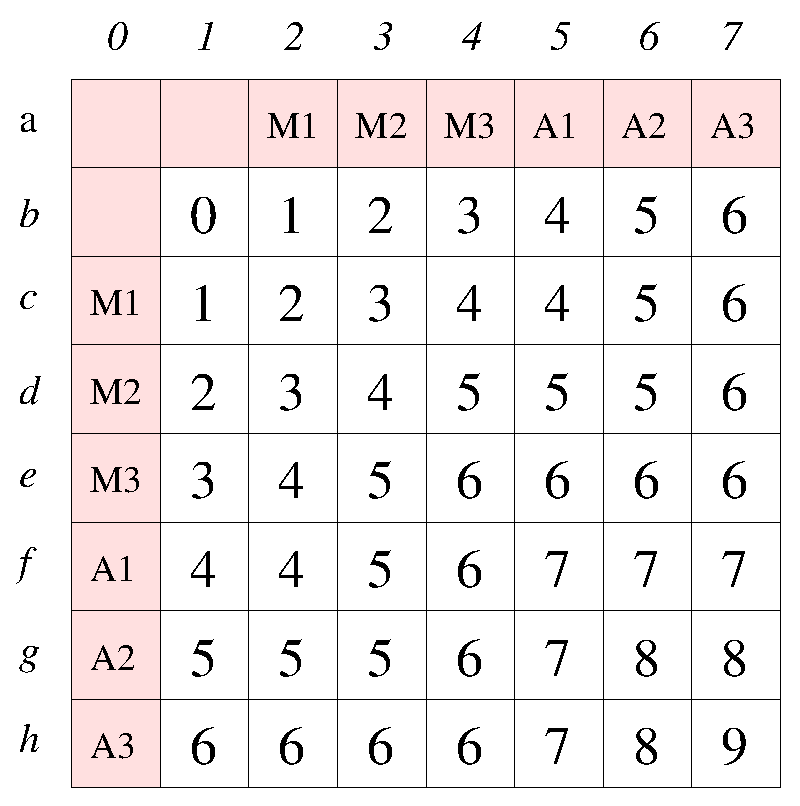
\includegraphics[width=0.3\textwidth]{figs/alloc.eps}
        }
        \hfill
        \subfigure[Stage 2: scoring table filling]
        {
            \label{fig:alloc:2}
            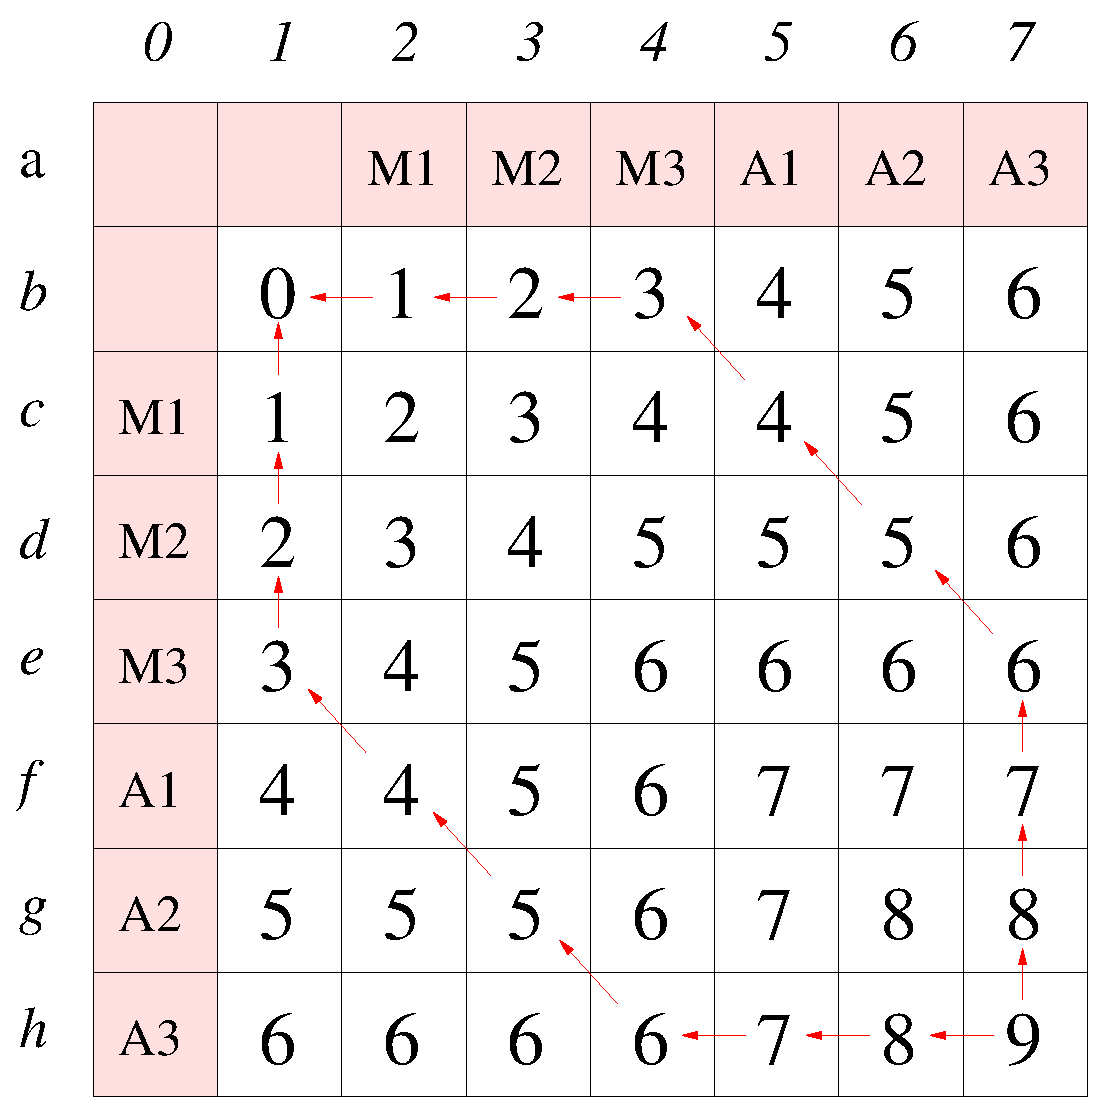
\includegraphics[width=0.3\textwidth]{figs/alloc2.eps}
        }
        \hfill
        \subfigure[Stage 3: backtracking]
        {
            \label{fig:alloc:3}
            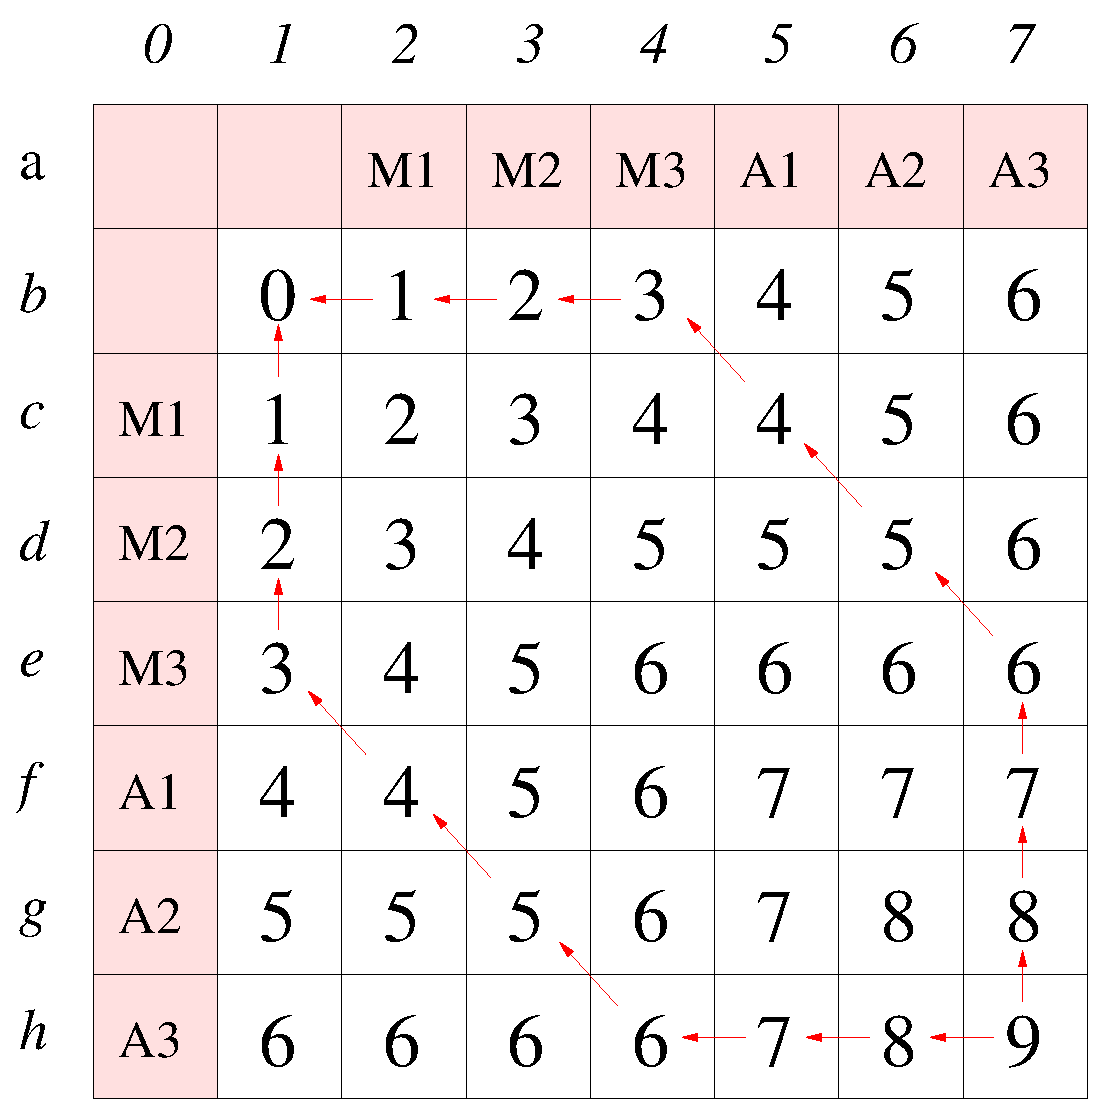
\includegraphics[width=0.3\textwidth]{figs/alloc3.eps}
        }
    \end{center}
    \caption{DP-based ALUs allocation}
    \label{fig:alloc}
\end{figure}

\indent
Another insight of Algorithm~\ref{alg:intra} is making use of binary tree characteristics.
Since any left subtree and its sibling can be processed in parallel,
the scheduler can still balance the workload for two threads by splitting two subtrees from the root even if only one $bt$ remains in HDFG, 
and thus ILP is kept.





